% Definiciones y constantes de estilo
% Clase del documento
\documentclass[a4paper,11pt,twoside,openright,titlepage]{book}

%
% Paquetes necesarios
%

% Símbolo del euro
\usepackage{eurosym}
% Codificación UTF8
\usepackage[utf8]{inputenc}
% Caracteres del español
\usepackage[spanish, es-tabla]{babel}
% Código, algoritmos, etc.
\usepackage{listings}
% Definición de colores
\usepackage{color}
% Extensión del paquete color
\usepackage[table,xcdraw]{xcolor}
% Márgenes
\usepackage{anysize}
% Cabecera y pie de página
\usepackage{fancyhdr}
% Estilo título capítulos
\usepackage{quotchap}
% Algoritmos (expresarlos mejor)
\usepackage{algorithmic}
% Títulos de secciones
\usepackage{titlesec}
% Fórmulas matemáticas
\usepackage[cmex10]{amsmath}
% Enumeraciones
\usepackage{enumerate}
% Páginas en blanco
\usepackage{emptypage}
% Separación entre cajas
\usepackage{float}
% Imágenes
\usepackage[pdftex]{graphicx}
% Mejora de las tablas
\usepackage{array}
% Mejora de los símbolos matemáticos
\usepackage{mdwmath}
% Separar figuras en subfiguras
\usepackage[caption=false,font=footnotesize]{subfig}
% Incluir pdfs externos
\usepackage{pdfpages}
% Mejoras sobre las cajas
\usepackage{fancybox}
% Apéndices
\usepackage{appendix}
% Marcadores (para el pdf)
\usepackage{bookmark}
% Estilo de enumeraciones
\usepackage{enumitem}
% Espacio entre líneas y párrafos
\usepackage{setspace}
% Glosario/Acrónimos
\usepackage[acronym]{glossaries}
% Fuentes
\usepackage[T1]{fontenc}
% Tablas con Multifila y Multicolumna
\usepackage{multirow}
% Bibliografía (Ordenacion, etc)
\usepackage{cite}

% Enlaces
\hypersetup{hidelinks,pageanchor=true,colorlinks,citecolor=Fuchsia,urlcolor=black,linkcolor=Cerulean}

% Euro (€)
\DeclareUnicodeCharacter{20AC}{\euro}

% Inclusión de gráficos
\graphicspath{{./graphics/}}

% Texto referencias
\addto{\captionsspanish}{\renewcommand{\bibname}{Bibliografía}}

% Extensiones de gráficos
\DeclareGraphicsExtensions{.pdf,.jpeg,.jpg,.png}

% Definiciones de colores (para hidelinks)
\definecolor{LightCyan}{rgb}{0,0,0}
\definecolor{Cerulean}{rgb}{0,0,0}
\definecolor{Fuchsia}{rgb}{0,0,0}

% Keywords (español e inglés)
\def\keywordsEn{\vspace{.5em}
{\textbf{\textit{Key words ---}}\,\relax%
}}
\def\endkeywordsEn{\par}

\def\keywordsEs{\vspace{.5em}
{\textbf{\textit{Palabras clave ---}}\,\relax%
}}
\def\endkeywordsEs{\par}


% Abstract (español e inglés)
\def\abstractEs{\vspace{.5em}
{\textbf{\textit{Resumen ---}}\,\relax%
}}
\def\endabstractEs{\par}

\def\abstractEn{\vspace{.5em}
{\textbf{\textit{Abstract ---}}\,\relax%
}}
\def\endabstractEn{\par}

% Estilo páginas de capítulos
\fancypagestyle{plain}{
\fancyhf{}
\fancyfoot[CO]{\footnotesize\emph{\nombretrabajo}}
\fancyfoot[RO]{\thepage}
\renewcommand{\footrulewidth}{.6pt}
\renewcommand{\headrulewidth}{0.0pt}
}

% Estilo resto de páginas
\pagestyle{fancy}

% Estilo páginas impares
\fancyfoot[CO]{\footnotesize\emph{\nombretrabajo}}
\fancyfoot[RO]{\thepage}
\rhead[]{\leftmark}

% Estilo páginas pares
\fancyfoot[CE]{\emph{\pieparcen}}
\fancyfoot[LE]{\thepage}
\fancyfoot[RE]{\pieparizq}
\lhead[\leftmark]{}

% Guía del pie de página
\renewcommand{\footrulewidth}{.6pt}

% Nombre de los bloques de código
\renewcommand{\lstlistingname}{Código}

% Estilo de los lstlistings
\lstset{
    frame=tb,
    breaklines=true,
    postbreak=\raisebox{0ex}[0ex][0ex]{\ensuremath{\color{gray}\hookrightarrow\space}}
}

% Definiciones de funciones para los títulos
\newlength\salto
\setlength{\salto}{3.5ex plus 1ex minus .2ex}
\newlength\resalto
\setlength{\resalto}{2.3ex plus.2ex}

% Estilo de los acrónimos
\renewcommand{\acronymname}{Glosario}
\renewcommand{\glossaryname}{Glosario}
\pretolerance=2000
\tolerance=3000

% Texto índice de tablas
\addto\captionsspanish{
\def\tablename{Tabla}
\def\listtablename{\'Indice de tablas}
}

% Traducir appendix/appendices
\renewcommand\appendixtocname{Apéndices}
\renewcommand\appendixpagename{Apéndices}

% Comando code (lstlisting sin cambio de página)
\lstnewenvironment{code}[1][]%
  { \noindent\minipage{0.935\linewidth}\medskip
    \vspace{5mm}
    \lstset{basicstyle=\ttfamily\footnotesize,#1}}
  {\endminipage}
  

%Definiciones de funciones EXTRA para los titulos
\newlength\salto
\setlength{\salto}{3.5ex plus 1ex minus .2ex}

\newlength\resalto
\setlength{\resalto}{2.3ex plus.2ex}

\newcommand{\lsection}[1]
                {\section{#1}
                \vskip-.9\resalto   %%%% Aquí reculo el posible salto por defecto de \section
                \hrule
                \vskip+.9\salto}  %%%% vuelvo ha realizar el salto (puedes poner otra vez el 90%)



% Definiciones de comandos
\newcommand{\nombreautor}{TODO: Nombre Apellido1 Apellido2}
\newcommand{\nombretutor}{TODO: NombreTutor Apellido1 Apellido2}
\newcommand{\nombretrabajo}{TODO: Título del Trabajo de Fin de Máster}
\newcommand{\fecha}{TODO: Fecha de entrega}
\newcommand{\master}{TODO: Máster}
% Descomentar si tu trabajo tiene un ponente
%\newcommand{\nombreponente}{TODO: Nombre del ponente}
% Descomentar si tu trabajo está asociado a un grupo de investigación
% \newcommand{\grupoInvestigacion}{TODO: Grupo de investigación}
\newcommand{\departamento}{TODO: Departamento}
\newcommand{\facultad}{Escuela Politécnica Superior}
\newcommand{\universidad}{Universidad Autónoma de Madrid}
\newcommand{\pieparizq}{TODO: Pie de página par}
\newcommand{\pieparcen}{Trabajo de Fin de Máster}
\newcommand{\logoizq}{Logo_EPS}
\newcommand{\logoder}{Logo_UAM}
\newcommand{\correo}{TODO: Correo de contacto}

% Glosario y acrónimos
\makeglossaries
% Acrónimos
%TFG
\newacronym[description={Graphic processing unit},longplural={unidades de procesamiento gráfico}]{gpu}{GPU}{unidad de procesamiento gráfico}
\newacronym{qos}{QoS}{Quality of Service}
\newacronym{dpi}{DPI}{Deep Packet Inspection}
\newacronym{dpdk}{DPDK}{Data Plane Development Kit}
\newacronym{dfa}{DFA}{Deterministic finite automaton}
\newacronym{hpet}{HPET}{High Precision Event Timer}
\newacronym{rtp}{RTP}{Real Time Protocol}
\newacronym[description={Field Programmable Gate Array},longplural={dispositivos de hardware programable}]{fpga}{FPGA}{dispositivo de hardware programable}
\newacronym[description={Network Interface Card},longplural={Interfaces de red}]{nic}{NIC}{Interfaz de red}
\newacronym[description={Núcleo lógico o Logical CORE}]{lcore}{LCORE}{logical core}

%TFM
\newacronym[description={Virtual Machine},longplural={máquinas virtuales}]{vm}{VM}{máquina virtual}
\newacronym[description={Virtual Network Function},longplural={funciones de red virtuales}]{nfv}{NFV}{función de red virtual}
\newacronym[description={Virtual Function},longplural={funciones virtuales}]{vf}{VF}{función virtual}
\newacronym[description={Internet Service Provider},longplural={proveedores de servicios de internet}]{isp}{ISP}{proveedor de servicios de Internet}
\newacronym[description={Software Defined Network},longplural={redes definidas por software}]{sdn}{SDN}{red definida por software}
\newacronym[description={Gigabit per second},longplural={Gigabits por segundo}]{gbps}{Gbps}{Gigabit por segundo}
\newacronym[description={Operative System},longplural={Sistemas operativos}]{os}{OS}{Sistema Operativo}
\newacronym[description={Solid-state drive},longplural={Discos de estado sólido}]{ssd}{SSD}{Disco de estado sólido}

% Glosario 

% TODO: Añadir aquí las definiciones del glosario
% Ejemplo de glosario
\newglossaryentry{cloud}{name={Cloud Computing},description={Se define la computación en la nube, como un conjunto de servicios que se encuentran en internet. Dichos servicios suelen estar descentralizados y repartidos en localizaciones y elementos físicos a los que usualmente no se tiene acceso}}

\newglossaryentry{cpu}{name={CPU},description={La tan conocida Unidad de procesamiento central, o CPU, se encarga de realizar la mayor parte de las tareas que realiza un ordenador de hoy en día. En las últimas arquitecturas, es también la encargada de coordinar diferentes dispositivos como la memoria o el bus PCIe.}}

\newglossaryentry{sriov}{name={SR-IOV},description={También conocida como \textit{Single Root I/O Virtualization}, SR-IOV~\cite{bib:introduccion:sriov} es una tecnología de virtualización que permite a un único dispositivo PCIe, mostrarse como diversas funciones virtuales (VF). Cada una de estas VF, puede conectarse a una máquina virtual, de forma que la compartición del dispositivo sea realizada por el propio hardware. Esto, minimiza el coste computacional de la máquina anfitriona, así como de las diversas máquinas virtuales que utilizan el dispositivo}}

\newglossaryentry{passthough}{name={Passthough},description={Se denomina Passthough, al mecanismo que tienen las máquinas virtuales para apoderarse por completo de un determinado dispositivo, ``desconectandolo'' de la máquina anfitriona. De esta forma, el sistema operativo invitado, es capaz de utilizar los drivers de forma nativa con el dispositivo y en principio con perdida de rendimiento 0}}

\newglossaryentry{virtio}{name={VirtIO},description={La tecnología VirtIO~\cite{russell2008virtio}, forma una parte importante de la tecnología de virtualización de KVM. El concepto de VirtIO, abarca desde los drivers de la máquina virtual, hasta los propios dispositivos virtuales generados por KVM. Un dispositivo VirtIO es, en esencia, una paravirtualización del dispositivo original}}

\newglossaryentry{mactiva}{name={monitorización activa},description={La monitorización activa consiste en la realización de una serie de medidas de una red, en donde dos o más nodos de la misma, intercambian un conjunto de paquetes. A partir de estos paquetes, se obtienen medidas como ancho de banda, jitter, latencia o cantidad de paquetes perdidos}}

\newglossaryentry{mpasiva}{name={monitorización pasiva},description={La monitorización pasiva consiste en la captura de tráfico en uno o varios puntos de la red. Analizando el tráfico capturado es posible obtener multitud de información, incluidos problemas a niveles de aplicación}}

\newglossaryentry{multicore}{name={multicore},description={Dentro de este contexto, la palabra \textit{multicore} hace referencia a los sitemas con más de una unidad de cómputo, ya sea porque hay más de un procesador completo, o se trate de un procesador con más de un \textit{core}}}

\newglossaryentry{core}{name={core},description={Entendemos como \textit{core}, como la unidad de procesamiento más básica de la que dispone nuestro sistema. Entendemos igualmente, que un \textit{core}, solo puede ejecutar un único hilo o proceso simultáneamente sin que su rendimiento se vea perjudicado}}


\newglossaryentry{zerocopy}{name={zero-copy},description={Hablamos de zero-copy, cuando una aplicación no necesita realizar ninguna copia de los datos (Normalmente de la memoria del kernel a la de usuario) para trabajar con ellos}}

\newglossaryentry{onecopy}{name={one-copy},description={Hablamos de one-copy, cuando una aplicación no requiere realizar una única copia de los datos (Normalmente de la memoria del kernel a la de usuario) para trabajar con ellos}}

\newglossaryentry{cache}{name={cache},description={Se suele llamar cache a una pequeña memoria de alta velocidad, que comunica una memoria lenta de tamaño muy superior y otro dispositivo. Por el principio de localidad y de temporalidad, almacenar los datos en una caché permite a, por ejemplo, microprocesadores, tener un acceso a los datos mucho más rápidamente}}

\newglossaryentry{vanilla}{name={vanilla},description={Se denomina a un elemento vanilla, cuando dicho elemento se encuentra en su estado original, sin modificaciones}}

\newglossaryentry{u}{name={U},description={Bajo el contexto de los equipos enracables, se denomina una U a la unidad básica de espacio que ocupa un equipo en un rack.}}

\newglossaryentry{raid0}{name={RAID 0},description={Se llama comunmente RAID a un grupo de discos duros que actúan en conjunto mostrándose al sistema operativo como un único disco duro. Un raid 0, es un caso específico en el cual todos los discos que forman el RAID, se encuentran al mismo nivel, es decir, no existe ningún disco que replique datos}}

\newglossaryentry{hypervisor}{name={hypervisor},description={Se denomina hypervisor a la capa virtual que conecta una máquina virtual con los diferentes dispositivos físicos de la máquina anfitriona. Este elemento, también es el encargado de la paravirtualización y de la virtualización completa de dispositivos}}

\newglossaryentry{huge}{name={HugePage},description={Un ordenador convencional divide la memoria del sistema en bloques alineados e indivisibles denominados páginas. Cada una de estas páginas pueda ser asignada a un proceso diferente o ser escrita a disco. De forma tradicional, estas páginas han tenido un tamaño de 4~KB, no obstante, manejar páginas tan pequeñas puede llegar a suponer una enorme sobrecarga para el sistema operativo. Por este motivo, los nuevos sistemas soportan páginas de 2~MB o incluso 1~GB. A estas dos últimas, se las conoce por el nombre de HugePages}}


%DOBLEGLOSARIOS:

\newglossaryentry{kvmg}{name={KVM},
    description={La tecnología KVM~\cite{bib:kvm} es una de las más populares en cuanto a virtualización se refiere, junto con su mayor competidor XEN. Esta tecnología se encuentra presente en el Kernel de Linux (en formato de módulo) y ofrece desde este nivel de ejecución la capacidad de virtualizar diferentes máquinas y dispositivos. Gracias a la tecnología actual de los procesadores (VT-X/AMD-V), esta virtualización puede llegar a ser transparente para la máquina virtualizada, además de ofrecer un aislamiento entre las diferentes máquinas virtuales y la propia máquina física}}
\newglossaryentry{kvm}{type=\acronymtype, name={KVM}, description={Kernel-based Virtual Machine}, first={máquina virtual basada en el Kernel (KVM)\glsadd{kvmg}}, see=[Glosario:]{kvmg}, firstplural={máquinas virtuales basadas en el Kernel (KVMs)\glsadd{kvmg}}}


\newglossaryentry{capexg}{name={CAPEX},
    description={El término inglés CAPEX, se refiere fundamentalmente a los gastos iniciales (o de actualización si es el caso), que son necesarios para poner en marcha un producto, o construir algo}}    
\newglossaryentry{capex}{type=\acronymtype, name={CAPEX}, description={CAPital EXpenditures}, first={gasto de capital inical (CAPEX)\glsadd{capexg}}, see=[Glosario:]{capexg}}


\newglossaryentry{opexg}{name={OPPEX},
    description={El término inglés OPPEX, se refiere fundamentalmente a los gastos que tiene un producto tras su contratación o compra}}    
\newglossaryentry{opex}{type=\acronymtype, name={OPPEX}, description={OPerational EXpenditures}, first={gasto de capital para operar (OPPEX)\glsadd{opexg}}, see=[Glosario:]{opexg}}


\newglossaryentry{numag}{name={NUMA},
    description={La arquitectura NUMA se basa en la descentralización de los recursos de un ordenador. De esta forma, cada procesador tiene su propia memoria y sus propios dispositivos. Si un procesador necesita acceder a los recursos de otro, debe pedirselos al procesador propietario de los mismos, el cual deberá interrumpir alguno de sus procesos para atender la petición. Estas peticiones, se realizan utilizando enlaces de altísima velocidad (como QPI), pero igualmente suelen ocasionar una degradación de rendimiento}}    
\newglossaryentry{numa}{type=\acronymtype, name={NUMA}, description={Non-Uniform Memory Access}, first={Acceso a Memoria No-Uniforme (NUMA)\glsadd{numag}}, see=[Glosario:]{numag}}


\newglossaryentry{mtug}{name={MTU},
    description={En el contexto de las redes de comunicaciones, se considera MTU al tamaño máximo que puede tener un paquete en un determinado enlace. Normalmente esta medida viene dada por una restricción del medio físico subyacente, no obstante, si no hubiese una limitación en la longitud de los paquetes, una aplicación podría abusar y emitir un paquete de tamaño infinito que colapsase indefinidamente la red}}    
\newglossaryentry{mtu}{type=\acronymtype, name={MTU}, description={Maximum Transmission Unit}, first={Unidad Máxima de Transmisión (MTU)\glsadd{mtug}}, see=[Glosario:]{mtug}}


\newglossaryentry{cpdg}{name={CPD},
    description={Un centro de datos (o Data Center), suele estar formado por varias habitaciones habilitadas para almacenar entre decenas y centenas de equipos. Estas salas se encuentran climatizadas, de forma que se mantenga una temperatura adecuada para el funcionamiento de los diferentes equipos. Estos centros de datos, suelen ofrecer a sus clientes luz y acceso a Internet a cambio de una cuota por cada U consumida}}    
\newglossaryentry{cpd}{type=\acronymtype, name={CPD}, description={Centro de procesamiento de datos}, first={Centro de procesamiento de datos (CPD)\glsadd{cpdg}}, see=[Glosario:]{cpdg}}


\newglossaryentry{hptlg}{name={HPTL},
    description={La librería HPTL partió de una primera implementación en mi trabajo fin de grado~\cite{rleira2013TFG}. Debido a la aparición de problemas de mantenibilidad y de configurabilidad, se decidió externalizar su uso como librería y publicarla en github~\cite{bib:hptl}}}    
\newglossaryentry{hptl}{type=\acronymtype, name={HPTL}, description={High Performance Timing Library}, first={librería de tiempo de alto rendimiento (HPTL)\glsadd{hptlg}}, see=[Glosario:]{hptlg}}




% Rerefencias
\bibliography{src/bibliografia}

% Inicio del documento
\begin{document}

% Elección del idioma (español)
\selectlanguage{spanish}

%
% Portada
%
\pagenumbering{gobble}
%
% Portada
%

% Universidad, Facultad
\begin{titlepage}
\selectlanguage{spanish}
\begin{center}
\textbf{\begin{huge}
\universidad \\
\end{huge}}
\bigskip 
\begin{LARGE}
\facultad \\
\end{LARGE}
\end{center}

\bigskip
\bigskip

%
% Imágenes (logos) izquierdo y derecho
%
\begin{figure}[h]
	\begin{center}
		\includegraphics[scale=0.35]{\logoizq}
    \hspace{1cm}
		\includegraphics[scale=0.4]{\logoder}
	\end{center}	
\end{figure}

\bigskip
\bigskip
\bigskip

% Máster
\begin{center}
\begin{large}
\textbf{\master}\\
\end{large}
\end{center}

\bigskip

\textbf{\begin{center}
\begin{huge}
\MakeUppercase{Trabajo de Fin de Máster}
\end{huge}
\end{center}}

\bigskip
\bigskip

% Nombre del TFG
\begin{center}
\textbf{\begin{large}
\MakeUppercase{\nombretrabajo}\\
\end{large}}
\end{center}

% Nombre del autor
\vspace{\fill}
\begin{center}
\textbf{\nombreautor}\\
% Tutor
\textbf{Tutor: \nombretutor}\\
% Ponente, si está definido en main.tex
\ifcsname nombreponente\endcsname
\textbf{Ponente: \nombreponente}\\
\fi

\bigskip

% Fecha
\textbf{\fecha}\\
\end{center}
\end{titlepage}

% Primera página
\pagenumbering{Alph}
\thispagestyle{empty}
\par\vspace*{\fill}
\begin{flushleft}
\begin{scriptsize}
\end{scriptsize}\end{flushleft}
\newpage
\thispagestyle{empty}
\begin{center}

% Nombre del trabajo
\textbf{\begin{large}
\MakeUppercase{\nombretrabajo}\\*
\end{large}}
\vspace*{0.2cm}
\vspace{5cm}

% Nombre del autor y del tutor
\large Autor: \nombreautor \\*
\large Tutor: \nombretutor \\*
\ifcsname nombreponente\endcsname
\large Ponente: \nombreponente\\
\fi

\vfill

% Grupo de investigación, departamento, facultad, universidad y fecha
\ifcsname grupoInvestigacion\endcsname
\grupoInvestigacion \\
\fi
\departamento \\
\facultad \\
\universidad \\
\vspace{1cm}
\fecha \\

\clearpage

\end{center}
\normalsize

\hypersetup{pageanchor=true}

% Estilo de párrafo de los capítulos
\setlength{\parskip}{0.75em}
\renewcommand{\baselinestretch}{1.25}
% Interlineado simple
\spacing{1}

%
% Agradecimientos
%
\pagenumbering{Roman}
\setcounter{page}{0}
\chapter*{Agradecimientos}

Son muchas a las personas a las que debería agradecer y poco el espacio en donde escribir.
A Juan Sidrach, por completar y mejorar esta plantilla en \LaTeX, así como a uno de sus creadores originales, Diego Hernando, el cual me ha apoyado siempre a lo largo de carrera y el Máster.
A Iván González, por haber sido un magnífico y comprensivo tutor y por ayudarme siempre en todo lo que ha podido. Gracias a el y a la ayuda de Victor Moreno, he podido finalizar con éxito este Trabajo Fin de Máster.
Al equipo de \href{http://www.handbe.com}{handbe}: Diego Hernando, Carlos Asensio y Paloma Domínguez, con los cuales he pasado muchas horas llevando a cabo nuestro proyecto y que también me han apoyado de múltiples formas.
A Raúl Martín, porque sin esos viajes en coche y nuestras conversaciones en el gimnasio, el año hubiese sido mucho más aburrido.

Y en general a todos los compañeros del grupo de investigación HPCN, ya que en mayor o menor medida han puesto su granito de arena a lo largo del Máster. Menciono especialmente a: Rubén García-Valcárcel, David Muelas, Mario Ruiz, José F. Zazo, Isabel García y a Sergio López Buedo.
De la misma manera agradezco el apoyo a todas y cada una de las personas que he conocido a lo largo de la carrera y del Máster, a mis amigos de toda la vida, a familiares y a Bea que de una u otra forma han estado conmigo a lo largo de este doble Máster haciéndolo más ameno y finalmente llevándome a escribir este TFM, y con él, a terminar mi doble Máster.

% Cita
%\begin{flushright}
%\textit{``TODO: Cita relevante''}
%TODO: Autor de la cita
%\end{flushright}
  

%
% Resumen
%
% Resumen en inglés
\chapter*{Abstract}

%\selectlanguage{english}
\begin{abstractEn}
%TODO: Resumen en inglés, 250-500 palabras.

\end{abstractEn}

% Palabras clave en inglés
\begin{keywordsEn}
Virtual network functions, packet capture, virtual machines, Intel DPDK, HPCAP
\end{keywordsEn}

% Resumen en español
\chapter*{Resumen}

\selectlanguage{spanish}
\begin{abstractEs}
%TODO: Resumen en español, 250-500 palabras.


\end{abstractEs}

% Palabras clave en español
\begin{keywordsEs}

\end{keywordsEs}


%
% Glosario
%
\printglossary[title=Glosario,toctitle=Glosario]
\printglossary[title=Acrónimos,toctitle=Acrónimos,type=\acronymtype]

% Estilo de párrafo de los índices
\setlength{\parskip}{1pt}
\renewcommand{\baselinestretch}{1}

%
% Tabla de contenidos
%
\tableofcontents
\listoftables
\listoffigures
\cleardoublepage

% Estilo de párrafo de los capítulos
\setlength{\parskip}{0.75em}
\renewcommand{\baselinestretch}{1.25}
% Interlineado simple
\spacing{1}
% Numeración contenido
\pagenumbering{arabic}
\setcounter{page}{1}

%
% Introducción
%
\chapter{Introducción}

Internet, es conocida como la red de redes. Cada año, más y más dispositivos se une a esta gran y colosal red. Una red, que desde hace mucho dejó de estar formada por solo ordenadores caseros y servidores, para ser un conjunto muy heterogéneo de dispositivos (como móviles~\cite{bib:introduccion:smartphone}, tablets e incluso neveras o relojes). Este gran aumento en la cantidad de dispositivos que conforman la red, ha sido parejo al aumento de la velocidad de la red, gracias a una gran cantidad de avances tecnológicos. Si bien, ahora es fácil poder disponer de un enlace simétrico a 100 o incluso a 300~Mbps en nuestros hogares, no podemos obviar que estos enlaces deben acabar por ser agregados en algún punto, convirtiéndose así en enlaces de 10, 40 o incluso 100~Gbps.

Aunque los enlaces de 100~Gbps comienzan a proliferan en los grandes \gls{isp}, aun son complicados de encontrar en otras grandes empresas. No obstante, si que es posible encontrar algunos enlaces e incluso subredes enteras a 10~Gbps. Mantener en funcionamiento redes de alta velocidad ($\geq$10~Gbps) requiere de una infraestructura de red con un alto \gls{capex} y un alto \gls{opex}. Dicha infraestructura, debe ser además monitorizada con regularidad para asegurar el correcto funcionamiento.

Toda la infraestructura de red así como el equipamiento de monitorización requieren, de forma tradicional, grandes y potentes máquinas dedicadas a realizar las típicas tareas de \textit{enrutado}, \textit{captura} o \textit{análisis de tráfico}, entre otras. No obstante, este tipo de necesidades no es nuevo. La mayoría de los servidores del mundo funcionaban en caros servidores dedicados, hasta la llegada del \gls{cloud}. El \gls{cloud} virtualiza los recursos clásicos de computación permitiendo a una compañía descentralizar de forma sencilla y barata sus servidores a lo largo del mundo, así como amoldarse en capacidad de cómputo a la demanda de sus clientes. Esto, inevitablemente minimiza el \gls{capex} y el \gls{opex} que una empresa debe afrontar para operar.

Internamente los diversos sistemas de \gls{cloud} utilizan \glspl{vm} para ofrecer sus servicios. Estas máquinas virtuales, deben a su vez conectarse entre sí y el resto del mundo dando lugar a redes virtuales. Sin embargo, virtualizar de forma completa una red, no permite que escale en velocidad y tamaño fácilmente, o no al menos, sin un alto coste y consumo de \gls{cpu}. Gracias a los avances en virtualización y a la aparición de la tecnología de \gls{sriov}, es posible virtualizar los diversos elementos de red dando lugar a las \glspl{nfv}.

\section{Objetivos}

TODO: Alcance del trabajo/proyecto

\section{Estructura del documento}

TODO: Descripción de la estructura del documento
%
% Estado del arte
%
\chapter{Estado del Arte\label{sec:estado_del_arte}}

Hoy en día, resulta complicado imaginar Internet como una red exclusiva de clientes y servidores. El fenómeno ``Internet of Things''~\cite{Atzori20102787} ha supuesto un cambio radical a hora de percibir que es Internet. Del mismo modo, que resulta difícil imaginarse a alguien sin un smartphone~\cite{bib:introduccion:smartphone} o sin acceso a Internet~\cite{bib:internet:growth}. Este crecimiento ha supuesto un equivalente aumento tanto en la velocidad como en tamaño de las redes internas de las empresas.

Para mantener una red de cierto tamaño en un buen estado, es necesario monitorizarla~\cite{de2013proactive}. Comunmente se habla de 2 tipos de monitorización: Activa y Pasiva. Cada tipo de monitorización ofrece una serie de ventajas e inconventientes. La \gls{mactiva}, permite a un administrador de red conocer el estado y la calidad de una red, pues este tipo de mediciones ofrece métricas como ancho de banda disponible, el jitter de la red (El cual es muy importante a la hora de transmitir contenido multimedia~\cite{dpdk:Leir1306,hernandomeasuring,garcia2014low}) o la latencia de la red entre dos extremos. No obstante, la monitorización activa afecta de mayor o menor forma al estado de una red, lo que puede perjudicar a la medida y por supuesto a los usuarios de la propia red. Estos efectos perjudiciales, pueden verse ampliados si la monitorización no se realiza mediante técnicas adecuadas~\cite{Ramos20111435}.

Por otro lado, la \gls{mpasiva} no sufre de los efectos perjudiciales de la \gls{mactiva}. Aunque este tipo de monitorización no es capaz de medir el jitter entre dos puntos de la red, ni tampoco la latencia a la que se ven sometidas determinadas comunicaciones, si ofrece otras muchas métricas relevantes. Para realizar este tipo de monitorización en una enlace de alta velocidad, es necesario un equipo de elevadas prestaciones para capturar el tráfico~\cite{dpdk:netfpga,dpdk:packetshader,moreno2012TFM,dpdk:victor:ref:1,dpdk:victor:ref:2,dpdk2015}.

Al disponer de todo el tráfico de un enlace, es posible obtener métricas de este, como pueden ser el ancho de banda del propio enlace, o de una determinada aplicación o usuario, la detección de intrusiones o incluso detección de malfuncionamiento de determinadas aplicaciones.
Aunque las posibilidades de la \gls{mpasiva} son muchas, tratar con toda esta cantidad de tráfico también supone una gran carga computacional. Por ello, existe multitud de investigación acerca de como escoger el tráfico que debe ser posteriormente almacenado o procesado.
Una de las aproximaciones más conocidas para segmentar el tráfico, es lo que se llama \textit{packet sampling}~\cite{1209210}. Este tipo de algoritmos intentan seleccionar el tráfico más relevante, de forma que sea posible obtener información estadística de ellos y a su vez reducir de manera drástica el número de paquetes por segundo que deben ser procesados. No obstante, utilizar \textit{packet sampling} tiene un cierto impacto en la medida~\cite{Brauckhoff:2006:IPS:1177080.1177101}, además de limitar el número de métricas interesantes que pueden obtenerse a partir de la \gls{mpasiva}.

Otros métodos de selección de tráfico, se basan en la selección por protocolo. Dado que existen miles de protocolos, es posible que de cara a realizar una monitorización solo nos preocupen algunos en concreto. Aunque identificar un protocolo a nivel de red o transporte es una tarea trivial, no lo es a la hora de identificar un protocolo a nivel de aplicación~\cite{dpdk:Leir1306}. Por este motivo, existen 3 formas diferentes de clasificar tráfico: por puerto, mediante clasificación estadística o mediante \gls{dpi}.
La clásica clasificación por puerto, nos brinda velocidad en la clasificación, pero no es útil al a hora de clasificar protocolos sin puertos conocidos, detectar atacantes o errores de configuración. La clasificación estadística por otro lado, nos brinda un compromiso entre fiabilidad y velocidad, lo que ha propiciado una elevada cantidad de investigación~\cite{dpi:critica:3,dpi:critica:7,dpi:critica:8,dpi:critica:13}. No obstante, la clasificación estadística requiere disponer de una muestra preliminar del tráfico a partir de la cual obtener un modelo que utilizar posteriormente. De igual modo, es complicado confiar en este tipo de métricas si se desea aplicar algún tipo de reacción activa como denegar a un usuario el acceso a un recurso, a pesar de que la métrica acierte en el 99\% de los casos.
En el caso de \gls{dpi}, es necesario aplicar una gran cantidad de cálculo para obtener el resultado~\cite{dpi:critica:10b}. Por ello, se han desarrollado aplicaciones de \gls{dpi} que recurren a diversos coprocesadores como \glspl{gpu}~\cite{dpi:gnort,dpdk:Leir1306} o \glspl{fpga}~\cite{dpi:tfm:6,dpi:tfm:7,dpi:tfm:8,dpi:tfm:11}.
La propia detección de protocolos, aporta suficiente información como para la construcción de firewalls~\cite{dpi:juancho:master,dpi:pedro:2}, detección de intrusiones~\cite{dpi:gnort}, corrección de \gls{qos}~\cite{dpdk:Leir1306} entre otras muchas aplicaciones.

En redes de altas velocidades, en muchos casos resulta poco verosímil trabajar a nivel de paquete y frecuentemente resulta poco interesante. Por este motivo, la extracción de la información de flujo con su correspondiente análisis se vuelve fundamental~\cite{fp:pedroth}. Aunque generar la información de cada uno de los flujos supone procesar igualmente cada uno de los paquetes, resulta un proceso computacionalmente más barato que una clasificación \gls{dpi}. Este procesado de flujos tiene una gran cantidad de desarrollo por detrás ya que facilita el análisis posterior de una red. El tratamiento de flujos es un tema extenso, desde los estándar de NetFlow~\cite{claise2004cisco,rt:netflow} e IPFIX~\cite{hofstede14surveys,claise2008specification}, hasta el desarrollo de herramientas para \gls{cpu}~\cite{mckeown2008openflow,kimCOMCOM06,garcia2014low,fp:pedroth} o para diversos coprocesadores~\cite{fp:marco}.

En definitiva, para poder analizar una red de forma pasiva, ya sea a través de la información de los flujos, o de la información referente a los protocolos de un paquete, es necesario un conjunto de herramientas capaz de capturar el tráfico a la tasa de la red que se desee monitorizar.

\lsection{Herramientas de captura}

Las redes de 10~Gbps no son nuevas.
Con el objetivo en mente de realizar una \gls{mpasiva} de al menos 10~Gbps, es importante


%%OLD%%
Tal y como se mencionó en el capítulo anterior la realización de una sonda clasificadora está sometida a una serie de problemas.
Tradicionalmente, uno de los problemas fundamentales en redes ha sido obtener el máximo rendimiento de una tarjeta de red.
Para solucionar este problema había que recurrir a la construcción o modificación de un driver y en algunos casos extremos a un \gls{fpga}~.
Gracias a la aparición y apertura de Intel~\gls{dpdk}, estos problemas han sido simplificados en gran medida~\cite{dpdk:whitepaper:whydpdk}.

%%NEW%%
Realizar un proceso de captura a alta velocidad en un ordanador convencional, supone atravesar toda la pila de red de un sistema operativo, lo que de forma inevitable nos supone una degradación del rendimiento y en el caso de redes de $\geq$10~Gbps, un impedimento a la hora de capturar todo el tráfico. Para solventar este problema, se han desarrollado multitud de herramientas y hardware dedicado. Dos claros ejemplos de hardware dedicado son los procesadores de red Tilera~\cite{bib:tilera} y las FPGAs, en especial con su popular proyecto NetFPGA~\cite{dpdk:netfpga}. No obstante, trabajar con este tipo de harware supone un alto coste de programación, pues los sistema tienen una complejidad elevada. Por el otro lado, estos sistemas permiten realizar algunas tareas que en software serían mucho más complejas o incluso inviables. Algunos de los trabajos más interesantes en estas plataformas son: 
[]\cite{zazo2014tnt10g}


\lsection{Tecnologías de virtualización}


%%SDN!?

%
% Diseño
%
\chapter{Diseño\label{chap:disenho}}

TODO: Diseño del proyecto

%
% Desarrollo
%
\chapter{Pruebas\label{sec:desarrollo}}

El objetivo de este capítulo es mostrar tanto las pruebas realizadas como la metodología seguida para obtener los resultados.
Para poder entrar en detalle, en las pruebas, es necesario hacer un repaso de los dispositivos hardware y software que se encuentran disponibles. Una vez conocidos, es posible definir una metodología de pruebas, así como una descripción de las mismas en los diferentes entornos.

\lsection{Entorno de Desarrollo\label{sec:entorno}}

Escoger un entorno de desarrollo y pruebas adecuado, supone realizar multitud de comparativas y pruebas entre los diferentes elementos disponibles, tanto a nivel software, como a nivel hardware.
Poner a prueba todos y cada uno de los posibles elementos supone un reto en cuanto a coste monetario como en tiempo, y dado que tanto el presupuesto como el tiempo de realización del doble trabajo fin de máster son finitos, se ha partido del siguiente equipamiento facilitado por el grupo de investigación HPCN.

\subsection{Equipamiento de prueba utilizado\label{sec:equipamiento}}

El equipamiento de prueba utilizado costa de 3 elementos fundamentales: Captura de tráfico, emisión de tráfico y el tráfico emitido como tal.
Todos estos elementos son de vital importancia a la hora de realizar una comparativa, pues tan importante es el proceso de captura, como que los datos recibidos hayan sido emitidos correctamente. Estos datos, por otro lado, deben representar algún tráfico significativo para las pruebas, ya sea un caso extremo, o un caso realista. Cada una de estas partes es explicada con detalle a continuación:
\\
\\

\subsubsection{Equipo de captura y desarrollo}

El equipo de captura y desarrollo es conocido internamente por el nombre de \textit{Nrg}.
Esta sonda de captura, está compuesta por una arquitectura de tipo \gls{numa} con dos procesadores \textit{Intel Xeon E5-2630} a una velocidad de 2.6~Ghz cada uno.
Ambos procesadores se encuentran conectados a 2 tarjetas de memoria de 8~GB cada una, haciendo un total de 32~GB para todo el sistema.
Este equipo cuenta con diversos PCIe generación 3 que permiten transferencias de datos de hasta casi un 1~GBps por cada linea PCIe. El equipo cuenta con los siguientes dispositivos PCI:

\begin{itemize}
\item \textbf{Tarjeta gráfica Nvidia Tesla K40C}: A pesar de no haber sido utilizada la tarjeta gráfica a lo largo de las pruebas o el desarrollo, parece interesante mencionar su presencia en el bus PCIe.

\item \textbf{Tarjeta de red Ethernet Mellanox MT27500 (ConnectX-3)}: Esta tarjeta es capaz de establecer velocidades de enlace de entre 40 y 56~Gbps. Aunque inicialmente se pretendía probar esta tarjeta, Intel~\gls{dpdk} no publicó los drivers para explotar esta tarjeta hasta la versión 2.0, la cual fue publicada en abril de 2015. De igual modo, no disponemos de ningún emisor de tráfico fiable capaz de saturar este enlace, ni tampoco la capacidad de realizar el almacenamiento a disco a esta tasa de red sin realizar algún tipo de filtrado de tráfico. Hasta donde llega mi conocimiento, no existe (aparte del nuevo driver de Intel~\gls{dpdk} y el driver nativo) ninguna aplicación similar contra la que comparar resultados. Por todo esto, el uso de esta tarjeta ha sido descartado al encontrarse fuera del marco de este trabajo. Esta tarjeta conecta la máquina de captura con la máquina llamada \textit{Onelab3}.

\item \textbf{Tarjeta de red Ethernet Intel I350}: Esta tarjeta dispone de dos \glspl{nic} a 1~Gbps cada una. Dado la máquina de captura se encuentra inaccesible físicamente, se ha utilizado esta tarjeta como medio para el acceso remoto, así como el acceso a diferentes recursos y paquetes de Internet.

\item \textbf{Tarjeta de red Ethernet Intel 82599ES}: Esta tarjeta dispone de dos \glspl{nic} SFP+ a 10~Gbps cada una. El chipset \textit{82599ES} es compatible con la mayoría de capturadores de bajo coste actuales, por lo que la convierte en el dispositivo predilecto de cara a realizar una comparativa de rendimiento. Además, soporta diferentes modos de virtualización (\gls{passthough} y \gls{sriov}), permitiendo de esta forma alcanzar los objetivos planteados en este trabajo. Las dos interfaces de la tarjeta se encuentran conectadas al emisor de tráfico (llamado \textit{Dagda}), el cual será explicado más adelante.

\item \textbf{Controladora MegaRAID SAS-3 3108}: Dadas las limitaciones del chasis de la sonda de captura, la controladora RAID es capaz de gestionar hasta un máximo de 12 discos duros. Estos discos duros, pueden conformar desde un único Raid 0, hasta un conjunto de diferentes tipos de Raid. 
\end{itemize}

%seria interesante preguntar a victor por paper de referencia
Una vez observados los diferentes dispositivos disponibles, parece interesante realizar un inciso en la controladora raid.
Si bien puede gestionar hasta 12 discos duros, el precio de estos no es en absoluto despreciable.
En este caso, se parte de discos mecánicos \textit{Hitachi HUA 72303} (especiales para servidores) con 3~TB de capacidad cada uno.
El precio actual aproximado de estos discos duros oscila entorno a los \textit{310€}, elevando el coste de almacenamiento a más de \textit{3700€}.
Por este motivo, determinar cual es la cantidad de discos duros necesarios para cada escenario es de vital importancia de cara a reducir el coste de la sonda de captura.


\subsubsection{Equipo de emisión de tráfico}

Existen multitud de herramientas de emisión de tráfico.
Una de las herramientas clásicas es \href{http://tcpreplay.appneta.com/}{TCPReplay}.
Dicha herramienta parte de un fichero estándar \textit{PCAP} y lo transmite por una determinada interfaz de red. TCPReplay, proporciona cierto valor añadido, ya que puede regular la velocidad de transmisión entre otras muchas cosas. No obstante, esta herramienta al igual que la mayoría de emisores de tráfico clásicos (Como pktgen, etc), no es capaz de emitir tráfico a 10~Gbps, aun si este se encuentra en memoria. Esto se debe a que las herramientas de transmisión y generación de tráfico utilizan la pila de red completa del Kernel y los drivers \gls{vanilla} de las tarjetas de red.

De cara a solventar el problema de la generación y transmisión de tráfico, se han construido multitud de herramientas. Los generadores de tráfico software se basan en la reutilización de los drivers optimizados de captura como \gls{dpdk} o \textit{PacketShader}. No obstante, los emisores de tráfico software presentan serias limitaciones.
%
En el caso del emisor de \textit{PacketShader}~\cite{dpdk:packetshader}, se presentan ciertas irregularidades en la tasa de tráfico: emisión a ráfagas, problemas en los contenidos de los paquetes y en general problemas de estabilidad. De cara a hacer una comparativa de rendimiento y tasa de captura, estas irregularidades complicarían y harían fluctuar las medidas, por lo que este emisor fue descartado.
%
Por otro lado, Intel \gls{dpdk} proporciona una herramienta de emisión de tráfico bastante sofísticada conocida como \textit{Pktgen-\gls{dpdk}}~\cite{bib:dpdkpktgen}, la cual, poco a poco, se está convirtiendo en una conocida aplicación. 
La herramienta \textit{Pktgen} es capaz de saturar fácilmente 4 enlaces a 10~Gbps mediante tráfico sintético. Para conseguirlo, reserva las estructuras de los paquetes en memoria y las envía a cada una de las \gls{nic}. Esta herramienta, aunque útil para probar casos extremos, se ve perjudicada si lo que se desea es enviar tráfico almacenado previamente en un fichero. Debido al sobrecoste de las estructuras de los paquetes%
\footnote{Cada estructura de \gls{dpdk} almacena diversa información referente a un paquete. De cara a mantener la coalescencia de las cachés, estas estructuras cuentan con 2048 Bytes (La potencia de 2 más próxima a la \gls{mtu} de la red) para almacenar el payload del paquete.}%
 que utiliza \gls{dpdk}, no es posible almacenar más que unos pocos centenares de miles de paquetes por GigaByte. Aunque este número pueda aparentar ser muy grande, recordemos que en una red de 10~Gbps, se pueden llegar a mandar hasta casi 15 millones de paquetes por segundo (en caso de paquete mínimo), por lo que esta cantidad de paquetes representaría menos de una décima parte de segundo del tráfico del enlace.
 
En el otro lado, se encuentran los generadores hardware basados en \glspl{fpga}. Dentro del grupo de investigación HPCN ha sido desarrollado un potente y versátil generador de tráfico a 10~Gbps~\cite{zazo2014tnt10g}. Este generador, aporta un nivel de control en la transmisión de las tramas muy preciso, permitiendo simular, tanto cualquier situación de una red real, como casos extremos incluso a nivel físico.
Para lograr estas características, este sistema utiliza un formato especial de fichero denominado \textit{simple}. Este fichero es similar al formato PCAP, salvo porque almacena la cantidad de ceros que existen a nivel físico entre dos paquetes, lo que permite tener un elevado control y precisión durante la emisión. Dichos ficheros se encuentran en un Raid 0, de forma que un driver intermedio es capaz de acceder de forma eficiente a ellos y copiarlos en \glspl{huge}. Estas páginas son transferidas a la \gls{fpga} a través del bus PCIe. La \gls{fpga} emite el tráfico por una o varias de las diferentes \gls{nic} que posee. Como contrapartida, aunque la \gls{fpga} dispone de hasta 4 interfaces de 10~Gbps, solo es capaz de recibir hasta 10~Gbps por PCIe, por lo que como mucho podrá enviar el mismo tráfico simultáneamente por las diferentes \glspl{nic}. En la figura~\ref{fig:rafaDagda} se muestra un esquema del funcionamiento del generador y emisor de tráfico hardware.

\begin{figure}[!htb]
\centering
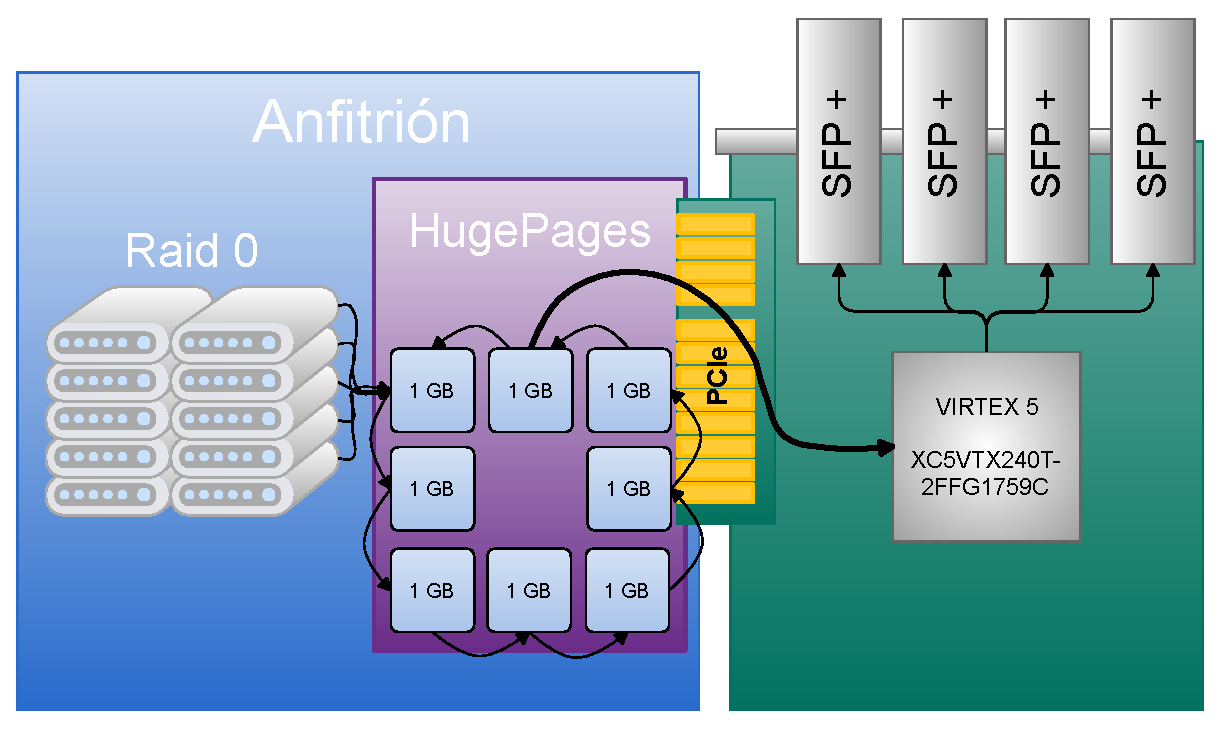
\includegraphics[scale=.6]{rafaDagda}
\caption{Arquitectura del emisor de tráfico}
\label{fig:rafaDagda}
\end{figure}

Tras escoger el generador de tráfico hardware, se definió un interconexionado de las diferentes máquinas que formarán parte de las diversas pruebas. La máquina encargada de la transmisión de tráfico (llamada \textit{Dagda}) se conecta mediante 2 interfaces de 10~Gbps a la máquina capturadora de tráfico (llamada \textit{Nrg}). La máquina de captura se encuentra a su vez conectada por un enlace de 40~Gbps con una máquina llamda \textit{Onelab3}. No obstante, y como se ha mencionado anteriormente, este enlace queda en desuso debido a la falta de software necesario para explotarlo adecuadamente. En la figura~\ref{fig:conexiones} se muestra gráficamente este interconexionado.

\begin{figure}[!htb]
\centering
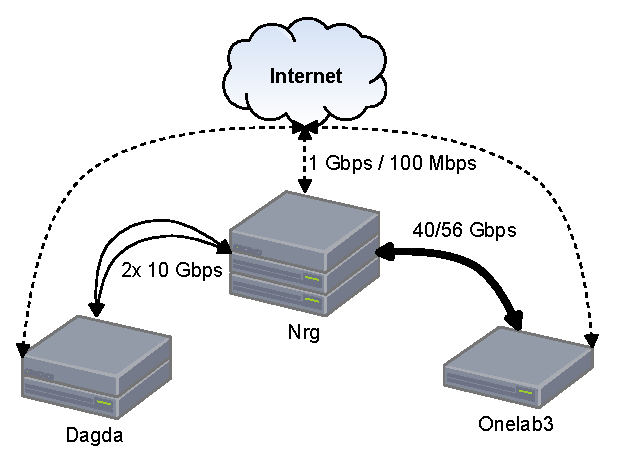
\includegraphics[scale=.8]{conexiones}
\caption{Conexionado del equipo de captura y desarrollo}
\label{fig:conexiones}
\end{figure}

\subsubsection{Tráfico emitido}

Una vez se ha decidido tanto el funcionamiento de la sonda de captura, como el hardware que se utilizará, es necesario definir el tráfico con el que se realizarán las evaluaciones, pruebas y comparativas. Para poder tener medidas útiles, es necesario poner al equipo de captura al límite, forzando y poniendo el sistema en el peor caso posible. No obstante, como se comentó en la introducción, resulta complicado encontrar enlaces completamente saturados, por lo que resulta interesante contar con tráfico representativo real.

Con el objetivo de cubrir ambos escenarios, se han utilizado los siguientes tipos de tráfico:

\begin{enumerate}

\item \textbf{Tráfico extremo}: Dentro del protocolo Ethernet, existen dos casos peores posibles: Un enlace en la que solo hay paquetes de 64 bytes y supone una tasa de 14.88 Millones de paquetes por segundo, o un enlace, en la que solo hay paquetes de tamaño 1500 y unos 800 mil paquetes por segundo.
En el primer caso, tan solo un 76\% de los bytes transmitidos%
\footnote{Los paquetes Ethernet tienen diversos campos, como el interframe gap o el preludio, que deben ser transmitidos pero no aportan ninguna información relevante. Por este motivo, dichos campos nunca son transmitidos por la tarjeta hacia el ordenador anfitrión y no pueden ser almacenados. En caso de que los paquetes sean muy pequeños, estos bytes ``ocultos'' se hacen relevantes.} %
 en el enlace son almacenados, mientras que en el segundo caso se almacenan entorno al 98\% de los bytes. Mientras que el primer caso requiere una mayor necesidad de computo para procesar un gigantesco número de paquetes, el segundo caso requiere de una mayor capacidad de escritura a disco.
Las herramientas proporcionadas por el generador de tráfico hardware escogido, son capaces de generar ambos escenarios extremos sin la necesidad de construir una traza a medida para la prueba.

\item \textbf{Tráfico Real}: Para poder obtener a tráfico real representativo a alta velocidad, es necesario recurrir a redes de grandes empresas o grandes nodos de interconexión de algún \gls{isp}. Esto causa, que la naturaleza de este tipo de tráfico suela ser confidencial o deba mantener ciertos requisitos de privacidad, por lo que, es complejo acceder a este tipo de muestras de tráfico.
Dentro de este contexto, la organización \href{http://www.caida.org/home/}{Caida}, captura tráfico en nodos que interconectan grandes ciudades de Estados Unidos. Tras realizar un proceso de anonimización\footnote{El proceso de anonimización consiste en truncar los paquetes eliminando la capa de aplicación.}, la organización Caida publica estas capturas de tráfico para su posterior uso por investigadores. Dentro de las trazas disponibles, se ha escogido una muestra unos 7 minutos de duración entre la ciudad de Seattle y la ciudad de Chicago el día 1 de octubre de 2014~\cite{caida2014}. Aunque esta traza está capturada en un enlace a 10~Gbps, la velocidad efectiva del tráfico ronda los 5~Gbps con un tamaño medio de paquete de unos 965 Bytes. De cara a realizar las pruebas y estresar un poco el sistema, se ha decidido acelerar transmisión de esta traza, reduciendo el tiempo entre los paquetes al mínimo posible.

\end{enumerate}

\subsection{Software utilizado\label{sec:sw}}

Encontrar el software apropiado para realizar un desarrollo es una tarea tediosa. Dado que el objetivo de este trabajo fin de máster es la realización de un motor de captura y almacenamiento de tráfico con Intel~\gls{dpdk} y la realización de una comparativa entre los diferentes métodos de captura en diferentes entornos de ejecución, es necesario plantear un entorno software aceptable para un posible cliente.
%
En el mundo empresarial, predomina el uso de las distribuciones de linux basadas en red hat o en suse. No obstante, la tecnología de virtualización, requiere de los últimos avances para poder ser explotada al máximo. Con esto en mente, la distribución de linux que mejor cumple estas condiciones es Fedora. Por este motivo, en la sonde captura se ha instalado un Fedora 20.

La mayoría de los entornos de virtualización de los que disponen las grandes compañías son: \gls{kvm}~\cite{bib:kvm}, XEN~\cite{bib:xen} o la versión profesional de VMWare~\cite{bib:vmware}. De cara a un presupuesto limitado, descartamos la opción de utilizar VMWare desde el principio. La decisión entre los hypervisores \gls{kvm} y XEN es algo más compleja pues son ambos sistemas muy utilizados, ambos son gratuitos y ambos se encuentran en auge. No obstante, se aprecia a la comunidad investigadora más enfocada en el entorno de \gls{kvm}, así como una gran cantidad de esfuerzo por parte de la comunidad de \gls{kvm} en el desarrollo de elementos y técnicas avanzadas de virtualización como \gls{virtio}. Por estos motivos, se ha escogido \gls{kvm} como método de virtualización.
%
Como optimización, dado que varios de los motores de captura hacen uso de las \gls{huge}, se ha configurado el sistema de virtualización \gls{kvm} para que reserve la memoria de las máquinas virtuales en \gls{huge} con el objetivo de que el rendimiento en las \glspl{vm} no se vea excesivamente afectado por problemas de paginación o problemas de cache. Las máquinas virtuales, a su vez, proveen \gls{huge} a los diferentes motores que se ejecutan en ellas.

Una vez que tenemos los más pilares básicos de nuestro sistema de captura, es necesario hacer un pequeño énfasis en lo que a funciones virtuales se refiere. Tal y como se ha explicado en capítulos anteriores, las funciones virtuales son a todos los efectos un dispositivo PCIe más. No obstante, las tarjetas Intel ofrecen diversas formas de crear y gestionar sus \glspl{nfv}. Por un lado, el driver \gls{vanilla} \textit{ixgbe}, permite indicar a la tarjeta que cree un número determinado de \glspl{nfv}, de una forma muy sencilla. No obstante, este tipo de funcionamiento delega todo el control de la función virtual a la tarjeta física, sin que la CPU intervenga en ningún caso en el trasiego de paquetes.
%
Por otro lado, el driver proporcionado por \gls{dpdk}, proporciona su propia forma de gestionar las funciones virtuales. Este paradigma, rompe ligeramente el concepto de \gls{vf}, ya que \gls{dpdk} requiere del uso de un determinado programa que de forma activa ayuda a la tarjeta a manejar las diferentes funciones virtuales. No obstante, este método obliga a la \gls{cpu} a trabajar, consumiendo, como mínimo, un \gls{core} completo. De cara a evaluar que método es el mejor, se han tenido en cuenta ambas aproximaciones y se detallan los resultados de la comparativa en la sección~\ref{sec:sriov}.

Dentro del software de captura de tráfico se ha decidido realizar una comparativa entre los siguientes motores: \gls{dpdk}, \textit{HPCAP}, \textit{PF\_RING}, y el driver \gls{vanilla} \textit{ixgbe} mediante el programa de captura \textit{TCPDump}~\cite{bib:tcpdump}. El resto de motores de captura han sido descartados para las pruebas, dado que su funcionamiento es muy similar entre sí, y ninguno de ellos es capaz de operar con~\gls{nfv}. Los motores de captura han sido explicados previamente en el capítulo~\ref{sec:estado_del_arte}.

\lsection{Metodología de las pruebas\label{sec:metod}}

Realizar todas y cada una de las pruebas que se describen en las siguientes secciones, supone un trabajo realmente tedioso y en un inicio muy manual. Si bien son importantes los resultados de las pruebas, es de igual importancia mantener un cierto protocolo a la hora de realizarlas asegurando su repetibilidad así como almacenar los resultados de forma organizada. Para llevar esto a cabo, se realizó un documento interno que incluía cada uno de los parámetros de los programas que se utilizaría, así como la forma de almacenar los resultados. A continuación se resumen algunas de las ideas que figuran en dicho documento:

\begin{itemize}
\item Crear un procedimiento de ejecución de los diferentes programas que conforman la prueba y seguirlo.
\item Todos los ficheros de resultados son almacenados en un documento de texto, siguiendo un mismo formato único independiente del motor de captura utilizado.
\item Organizar los ficheros de resultados en un árbol de carpetas, acorde al motor utilizado, el entorno de pruebas (virtual, físico, etc) y nombre del tráfico emitido.
\end{itemize}

El procedimiento de ejecución de una prueba, varía en función del entorno de la misma:

\begin{itemize}
\item \textbf{Procedimiento en entorno físico:}
\begin{enumerate}
\item Se reinicia la máquina con la configuración de memoria adecuada (En función de si el motor de captura utilizará o no \glspl{huge}.
\item Se resetea el generador de tráfico.
\item Se instancia el driver y programa de captura.
\item Se inicia la transmisión de tráfico por parte del generador (El tipo de tráfico varia en función de la prueba).
\item Al terminar la ejecución del programa de transmisión, se cierra el programa de captura y se almacenan los resultados.
\end{enumerate}

\item \textbf{Procedimiento en entorno virtual con \gls{passthough}:}
\begin{enumerate}
\item Se reinicia la máquina virtual con la configuración adecuada a la prueba.
\item Se resetea el generador de tráfico
\item Se instancia el driver en la máquina virtual y programa de captura.
\item Se inicia la transmisión de tráfico por parte del generador (El tipo de tráfico varia en función de la prueba).
\item Al terminar la ejecución del programa de transmisión, se cierra el programa de captura y se almacenan los resultados.
\end{enumerate}

\item \textbf{Procedimiento en entorno virtual con \gls{nfv}:}
\begin{enumerate}
\item Se instancia el driver encargado de la generación de \gls{nfv}.
\item Se reinicia la máquina virtual con la configuración adecuada a la prueba.
\item (Si procede) Se inicia el programa \textit{testpmd} de Intel~\gls{dpdk} en el anfitrión para apoyar con la gestión de \glspl{nfv}.
\item Se resetea el generador de tráfico
\item Se instancia el driver en la máquina virtual y programa de captura
\item (Si procede) Se configura el programa \textit{testpmd}
\item Se inicia la transmisión de tráfico por parte del generador (El tipo de tráfico varia en función de la prueba).
\item Al terminar la ejecución del programa de transmisión, se cierra el programa de captura y se almacenan los resultados de la máquina virtual y de la máquina anfitriona.
\end{enumerate}

\end{itemize}


\lsection{Pruebas en entorno físico\label{sec:fisico}}

\lsection{Pruebas en entornos virtuales\label{sec:virtual}}


\subsection{Usando Passthrough\label{sec:pt}}

\subsection{Usando SR-IOV\label{sec:sriov}}

%contar la diferencia de generación de NFV

\subsubsection{Comparativa de construcción de \glspl{nfv}}


\subsubsection{Comparativa de construcción de \glspl{nfv}}

%
% Resultados
%
\chapter{Resultados\label{chap:resultados}}

TODO: Pruebas y resultados

%
% Conclusiones
%
\chapter{Conclusiones\label{chap:conclusiones}}

TODO: Conclusiones sobre el trabajo realizado 

%
% Página en blanco
%
\cleardoublepage

%
% Bibliografía
%
\printbibliography[heading=bibintoc]

% No expandir elementos para llenar toda la página
\raggedbottom

%
% Apéndices
%
\appendix
\cleardoublepage
\addappheadtotoc
\appendixpage

%
% TODO: Apéndices del TFG
%
\chapter{Ejemplos de bloques y comandos útiles en LaTeX\label{sec:ejemplos}}
\section{Ejemplo de sección}

%
% Breve guía de comandos útiles para la memoria
%

% Citar una referencia
La DARPA creó el protocolo de Internet \cite{ipv4sta}.

% Citar un elemento del glosario
Citamos el acrónimo \gls{fpga}.

% Citar un elemento del glosario (primera letra en may´usculas)
\Gls{bitstream} es una secuencia de bits.

% Insertar una imagen con pie de página
\begin{figure}[htp!]
  \centering
  
\includegraphics[width=0.75\textwidth,clip=true]{Logo_UAM}
  \caption{Logo de la Universidad Autónoma de madrid.}
  \label{fig:logo_uam}
\end{figure} 

% Referenciar una etiqueta (label)
La figura~\ref{fig:logo_uam} se utiliza en la portada.

% Nueva página
\clearpage

% Añadir código fuente sin líneas
\begin{lstlisting}[label=algoritmo:quicksort,language=C,frame=single,caption=Algoritmo de ordenación Quicksort]
#include <stdio.h>
 
void quick_sort (int *a, int n) {
    int i, j, p, t;
    if (n < 2)
        return;
    p = a[n / 2];
    for (i = 0, j = n - 1;; i++, j--) {
        while (a[i] < p)
            i++;
        while (p < a[j])
            j--;
        if (i >= j)
            break;
        t = a[i];
        a[i] = a[j];
        a[j] = t;
    }
    quick_sort(a, i);
    quick_sort(a + i, n - i);
}
\end{lstlisting}

% Bloque de código inseparable
\begin{code}
#include <stdio.h>
 
void quick_sort (int *a, int n) {
    int i, j, p, t;
    if (n < 2)
        return;
    p = a[n / 2];
    for (i = 0, j = n - 1;; i++, j--) {
        while (a[i] < p)
            i++;
        while (p < a[j])
            j--;
        if (i >= j)
            break;
        t = a[i];
        a[i] = a[j];
        a[j] = t;
    }
    quick_sort(a, i);
    quick_sort(a + i, n - i);
}
\end{code}

% Fórmula dentro de una línea de texto
La ecuación de Euler ($e^{ \pm i\theta } = \cos \theta \pm i\sin \theta$) es citada frecuentemente como un ejemplo de belleza matemática.

% Fórmula independiente
\begin{equation}\label{eq:pythagoras}
a^2 + b^2 = c^2
\end{equation}


% Fin del documento
\end{document}
